
\section{Obsah CD nosiča} % (fold)
\label{sec:obsah_cd_nosi_a}
K práci je priložené CD, na ktorom sa nachádzajú implementované moduly spolu s demonštračnými aplikáciami a dokumentácia. Jeho súborová štruktúra je nasledujúca:

\begin{itemize}
  \item \textbf{/Dokument/}\\
    dokument a anotácie v slovenskom a anglickom jazyku\\
    \url{https://github.com/janantala/adaptive-web-design}

  \item \textbf{/IIT.SRC2014/}\\
    článok a poster prezentovaný na IIT.SRC2014\\
    \url{https://github.com/janantala/beyond-adaptive-web-design}

  \item \textbf{/source/angular-adaptive/}\\
    implementované moduly spolu s technickou dokumentáciou a inštalačnou príručkou\\
    \url{https://github.com/angular-adaptive}

  \item \textbf{/source/Gyrocopter/}\\
    rozšírenie do Chrome Developer Tools na emulovanie gyroskopu\\
    \url{https://github.com/janantala/Gyrocopter}

  \item \textbf{/source/speech-synthesis/}\\
    polyfill na syntézu reči spolu s technickou dokumentáciou a inštalačnou príručkou\\
    \url{https://github.com/janantala/speech-synthesis}

\end{itemize}

% section obsah_cd_nosi_a (end)


\newpage
\section{Technická dokumentácia a inštalačná príručka} % (fold)
\label{sec:technick_dokument_cia_a_in_tala_n_pr_ru_ka}

\begin{itemize}
  \item \textbf{adaptive-speech}
  \item \textbf{adaptive-scroll}
  \item \textbf{adaptive-motion}
  \item \textbf{adaptive-youtube}
  \item \textbf{adaptive-googlemaps}
  \item \textbf{adaptive-detection}
  \item \textbf{Gyrocopter}
  \item \textbf{speech-synthesis}
\end{itemize}

\newpage

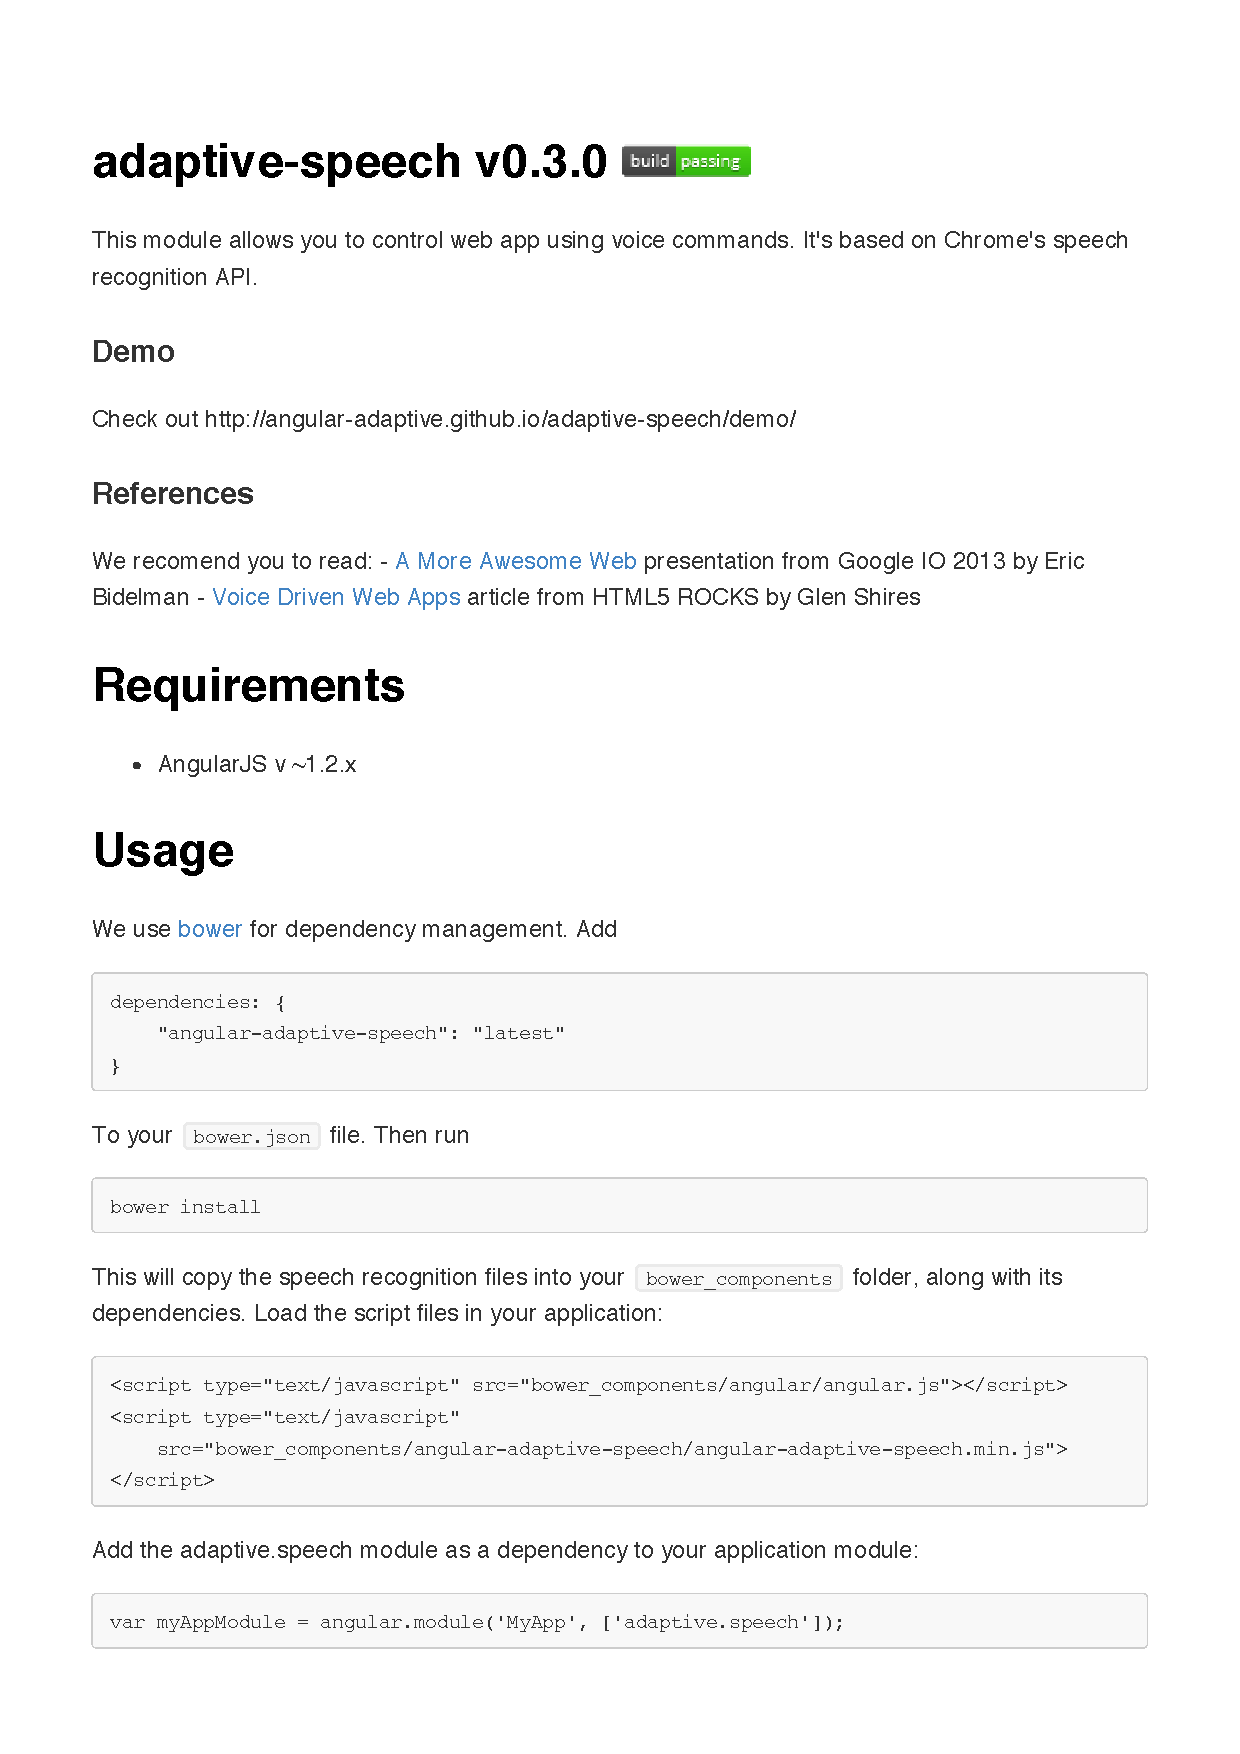
\includepdf[pages={1,2,3,4,5,6,7},scale=.8]{appendices/01-speech.pdf}
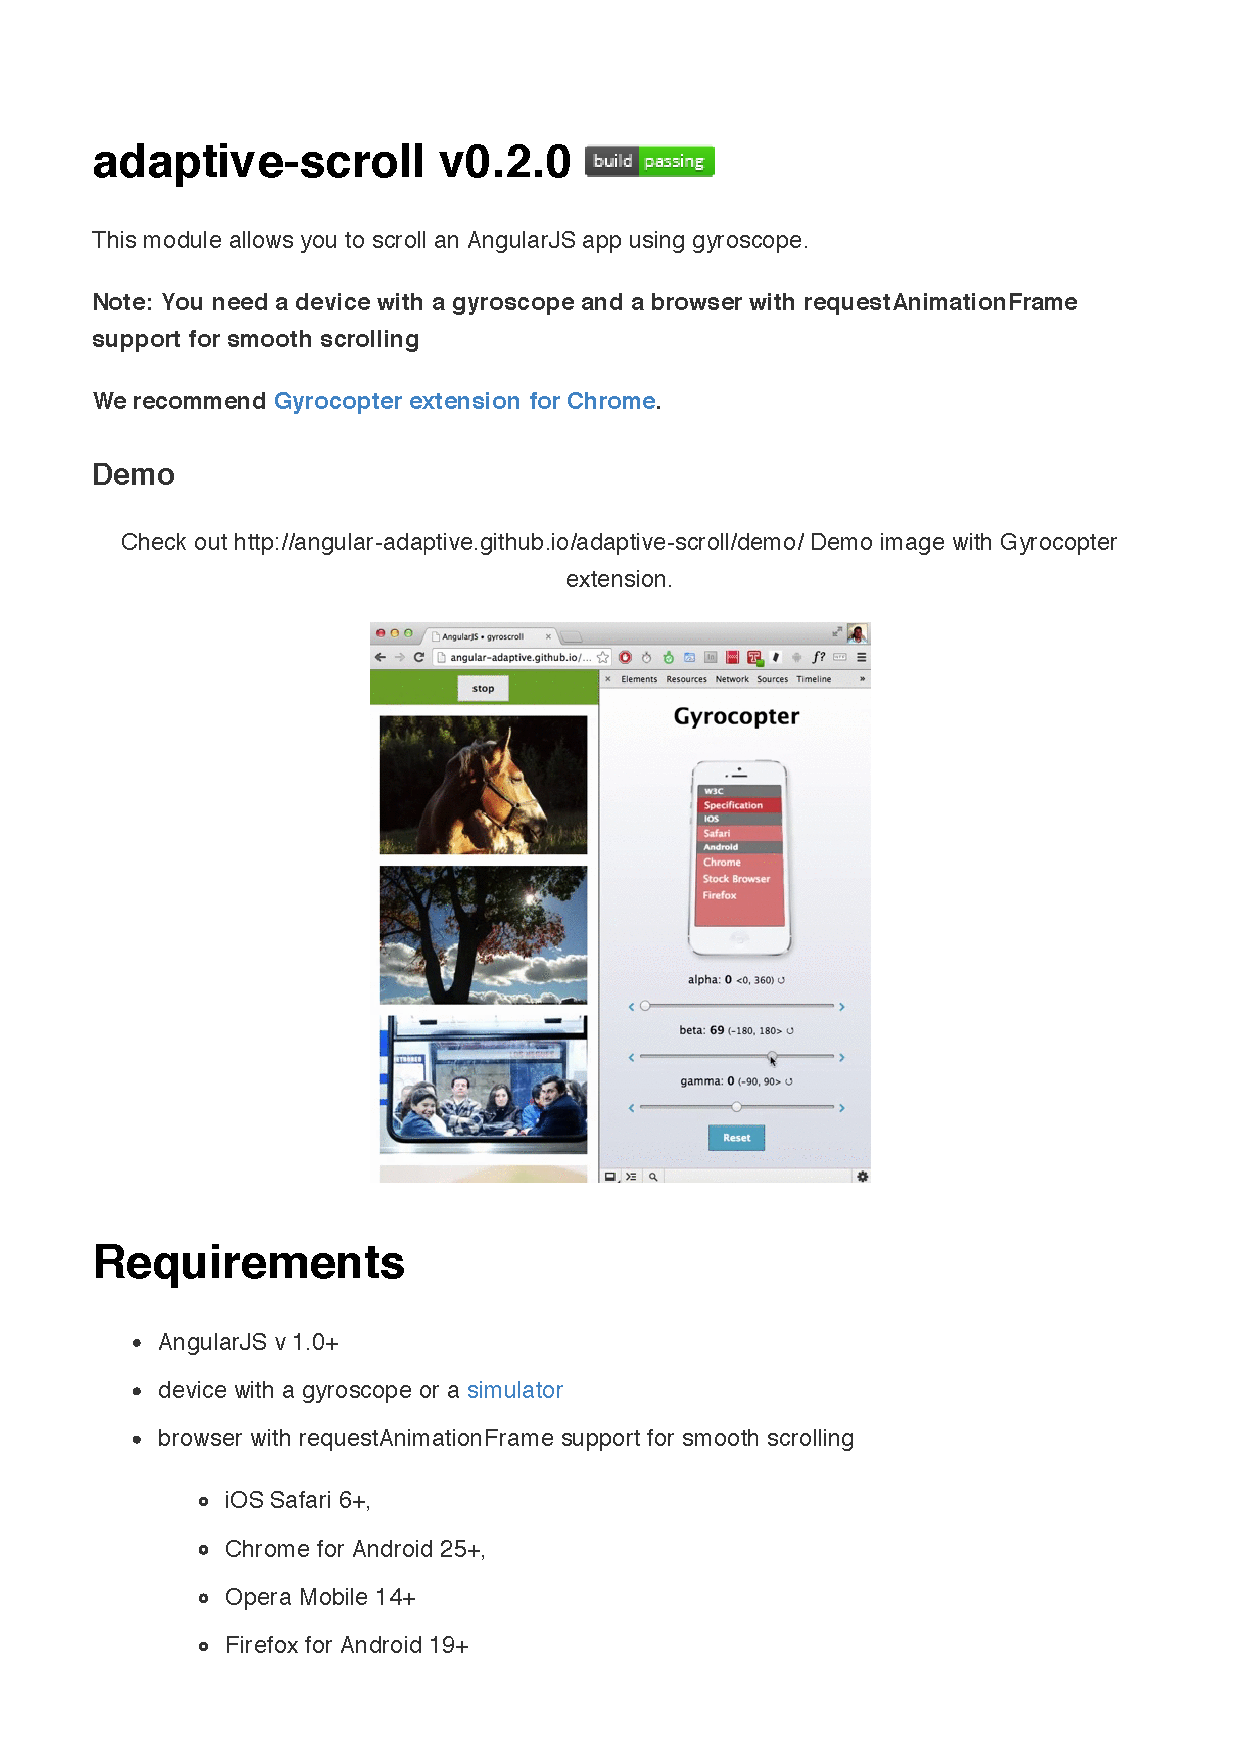
\includepdf[pages={1,2,3},scale=.8]{appendices/02-scroll.pdf}
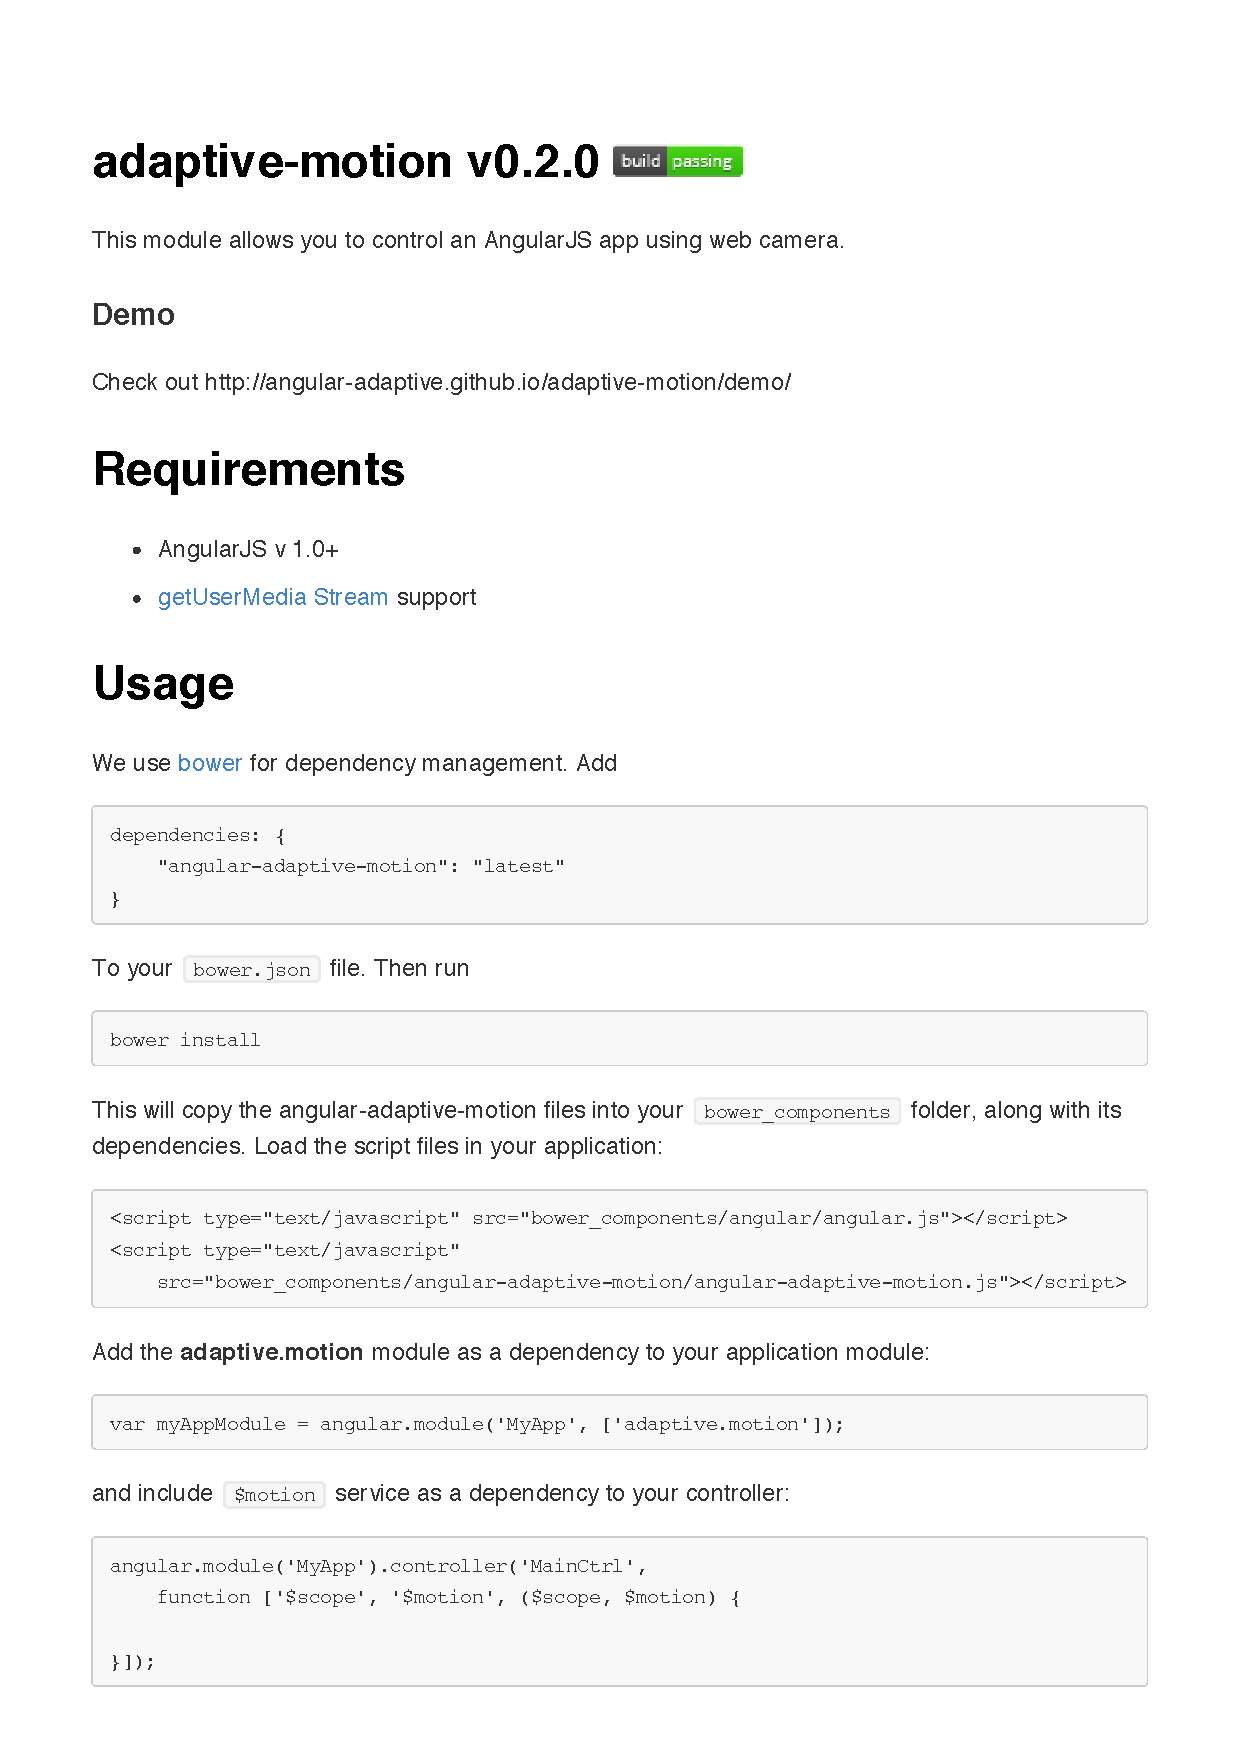
\includepdf[pages={1,2,3,4},scale=.8]{appendices/03-motion.pdf}
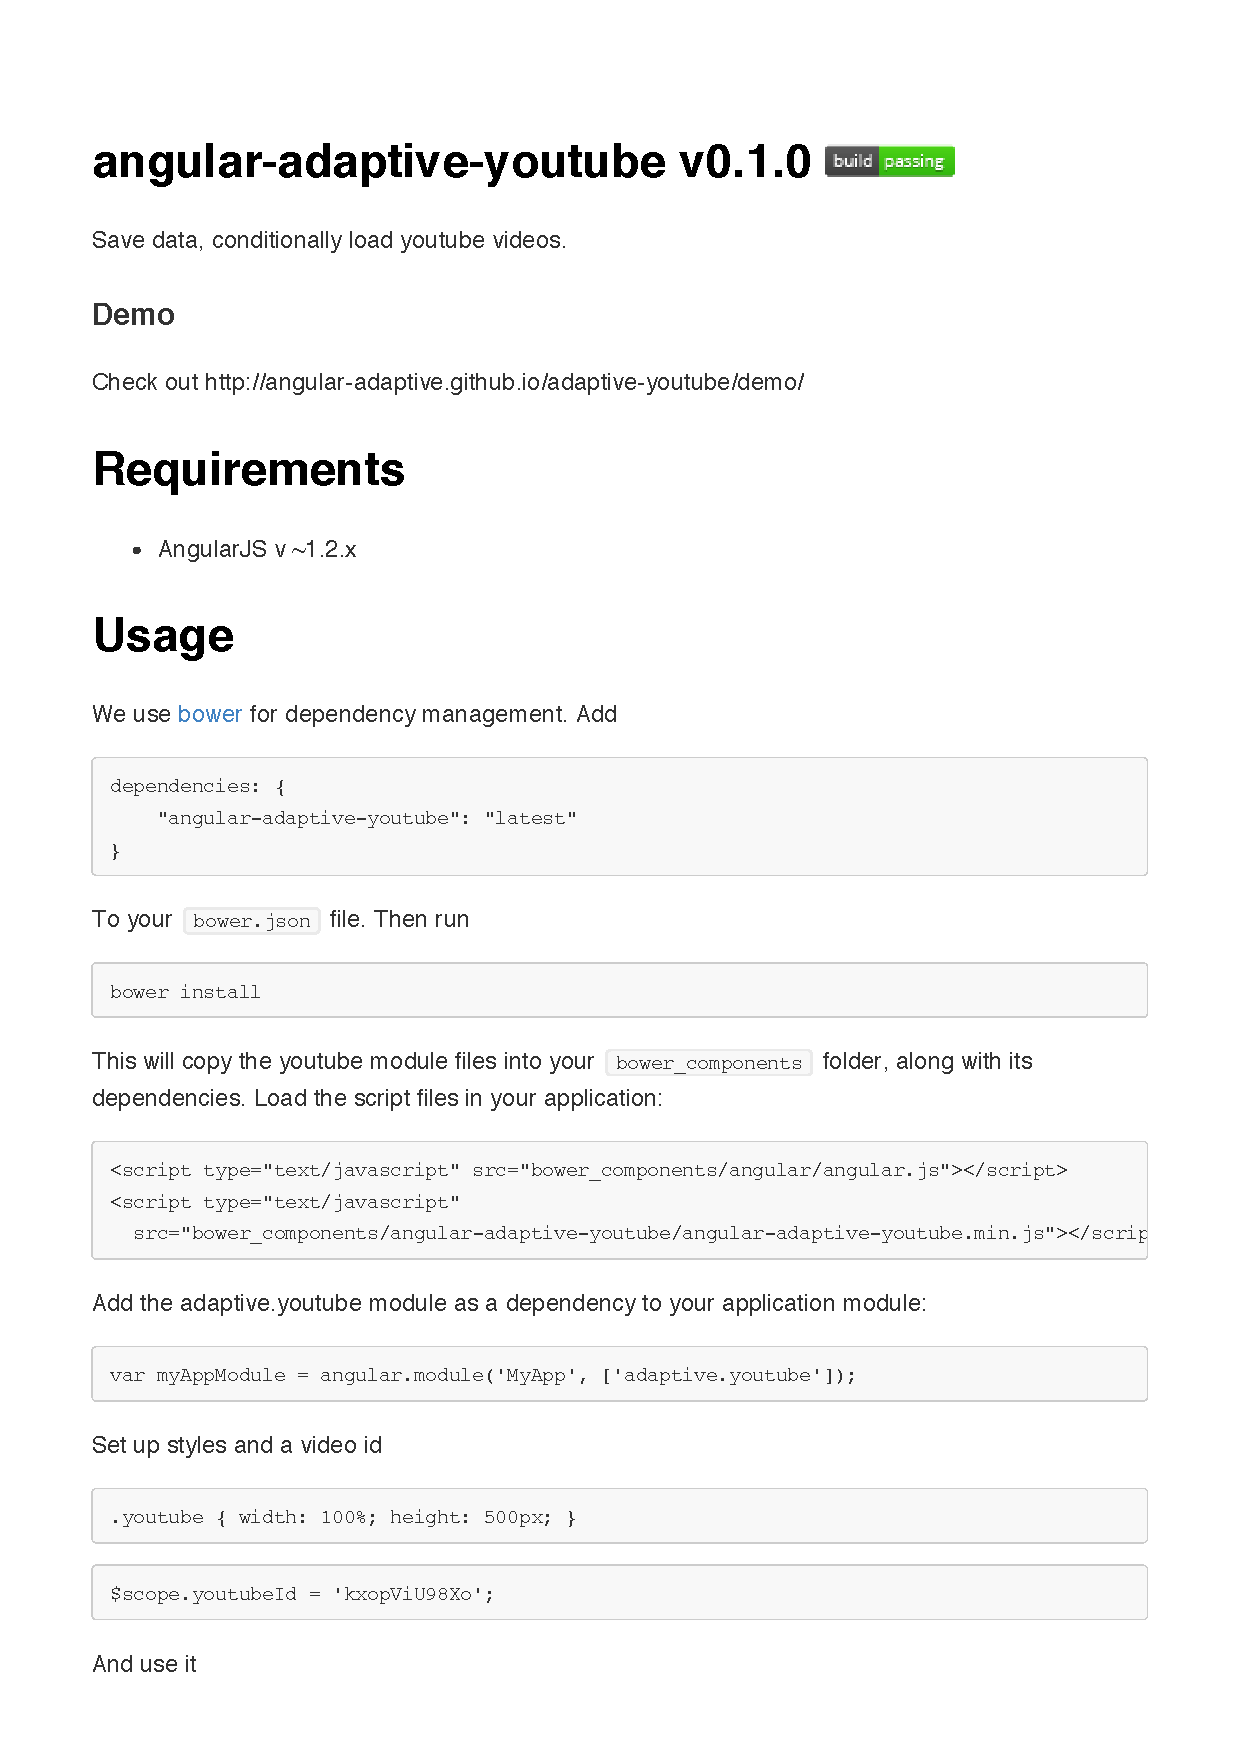
\includepdf[pages={1,2},scale=.8]{appendices/04-youtube.pdf}
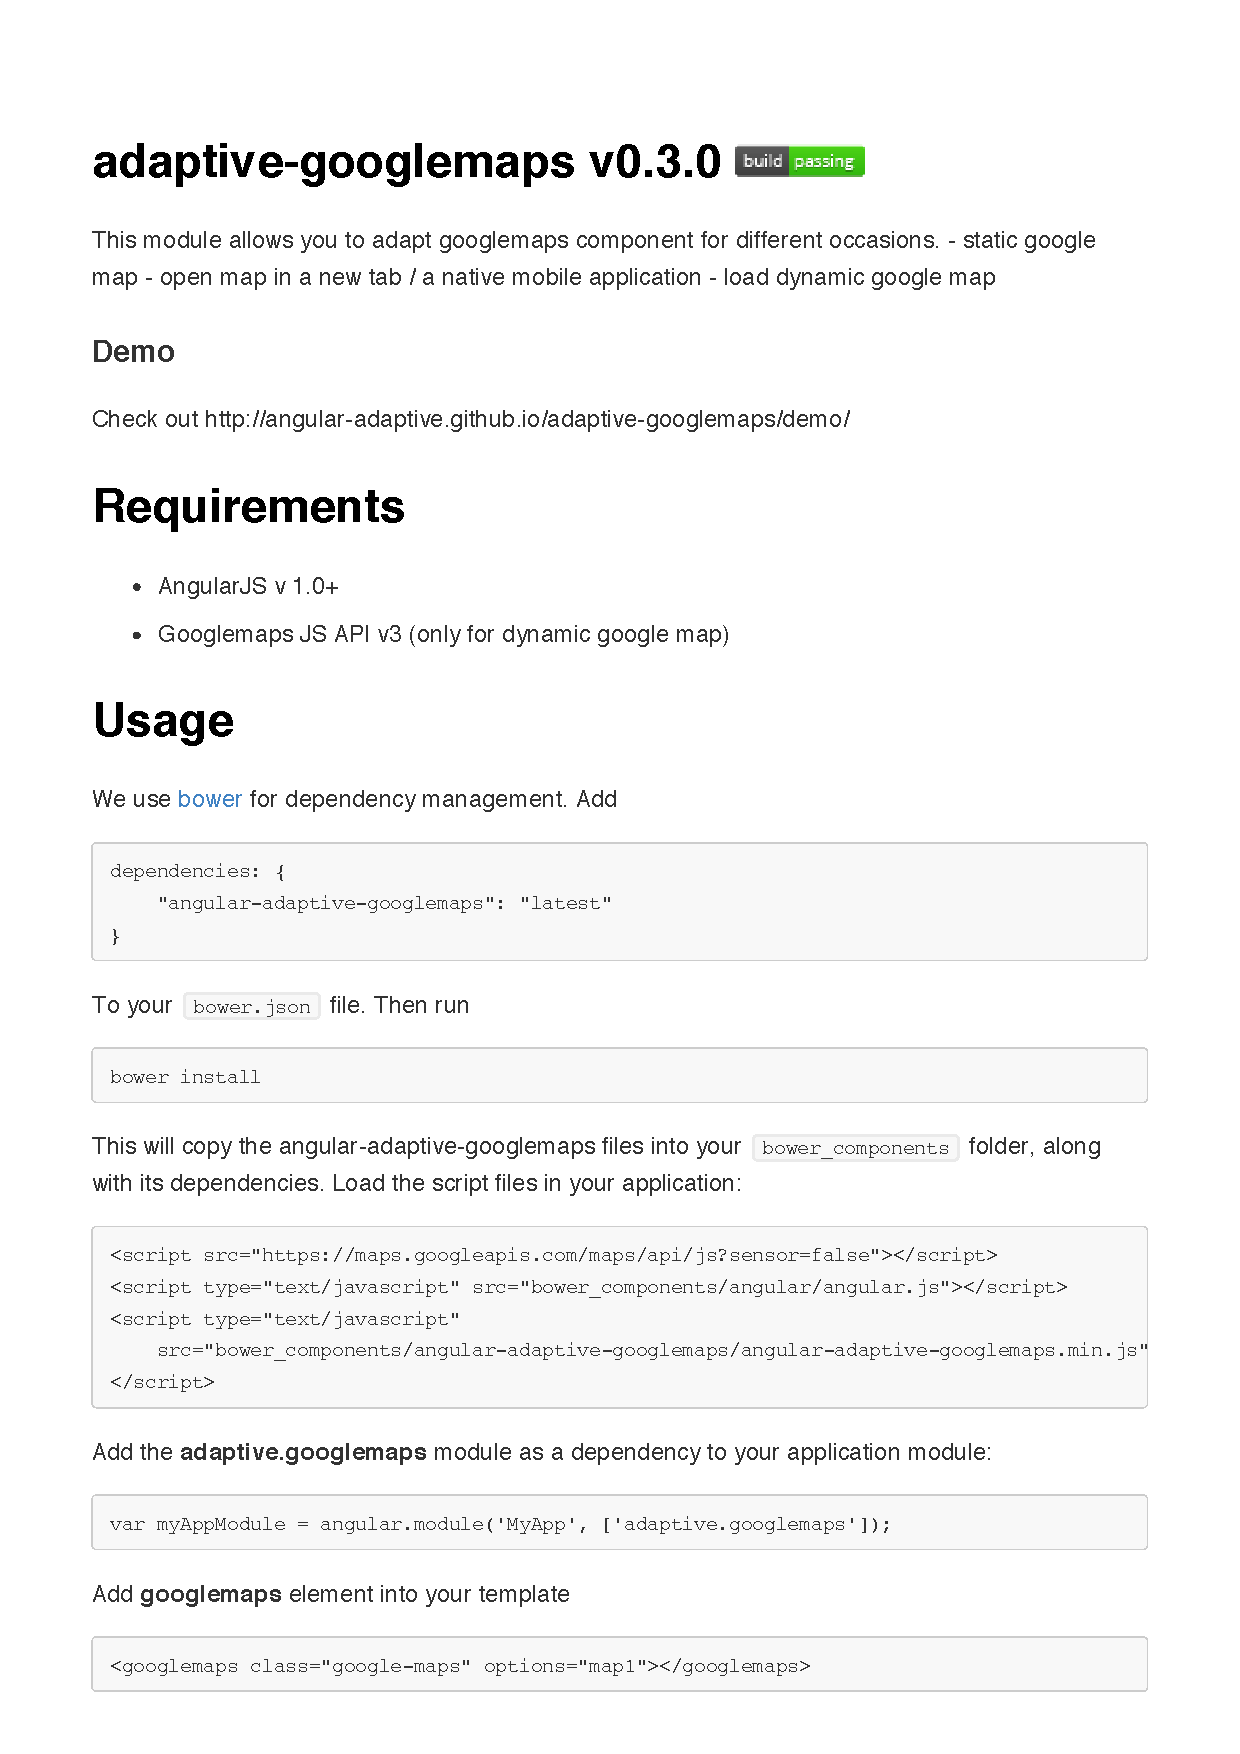
\includepdf[pages={1,2,3,4},scale=.8]{appendices/05-googlemaps.pdf}
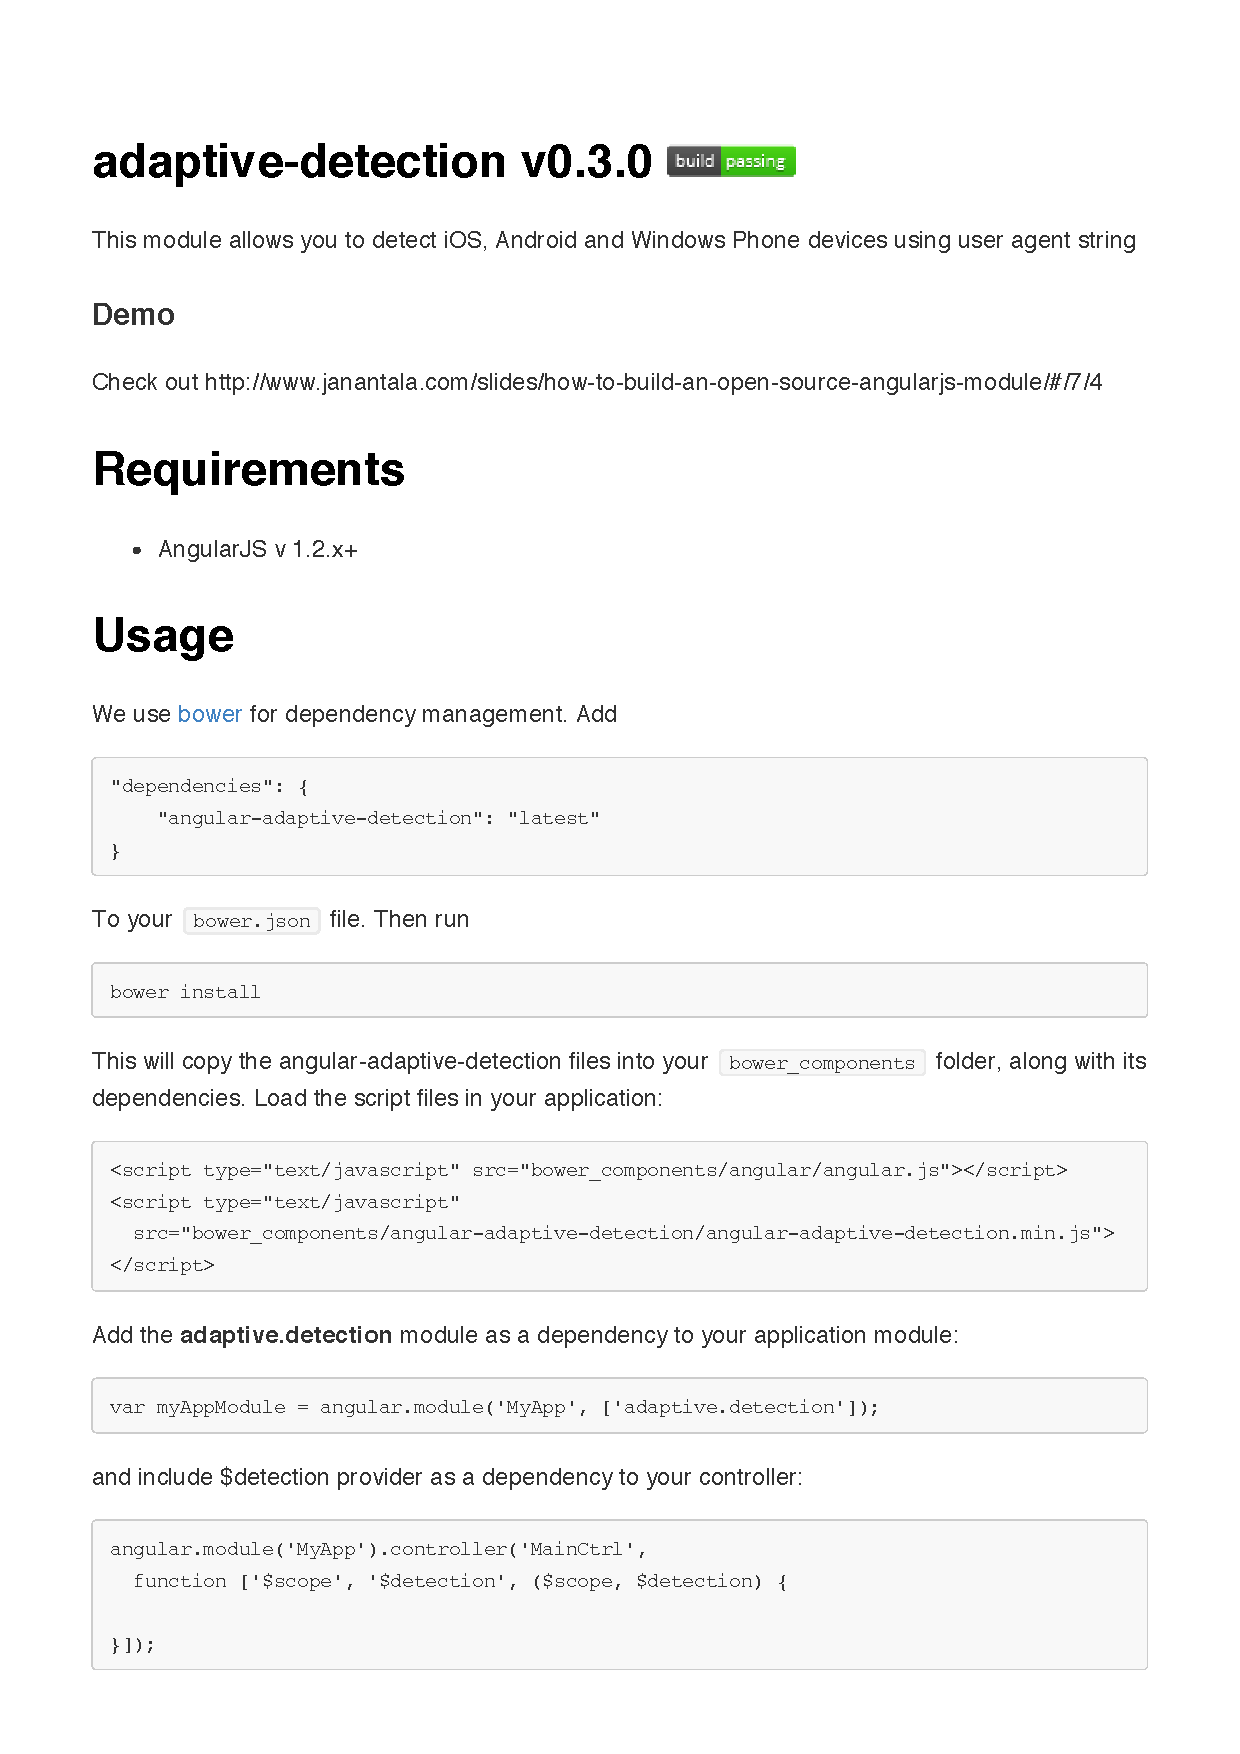
\includepdf[pages={1,2},scale=.8]{appendices/06-detection.pdf}
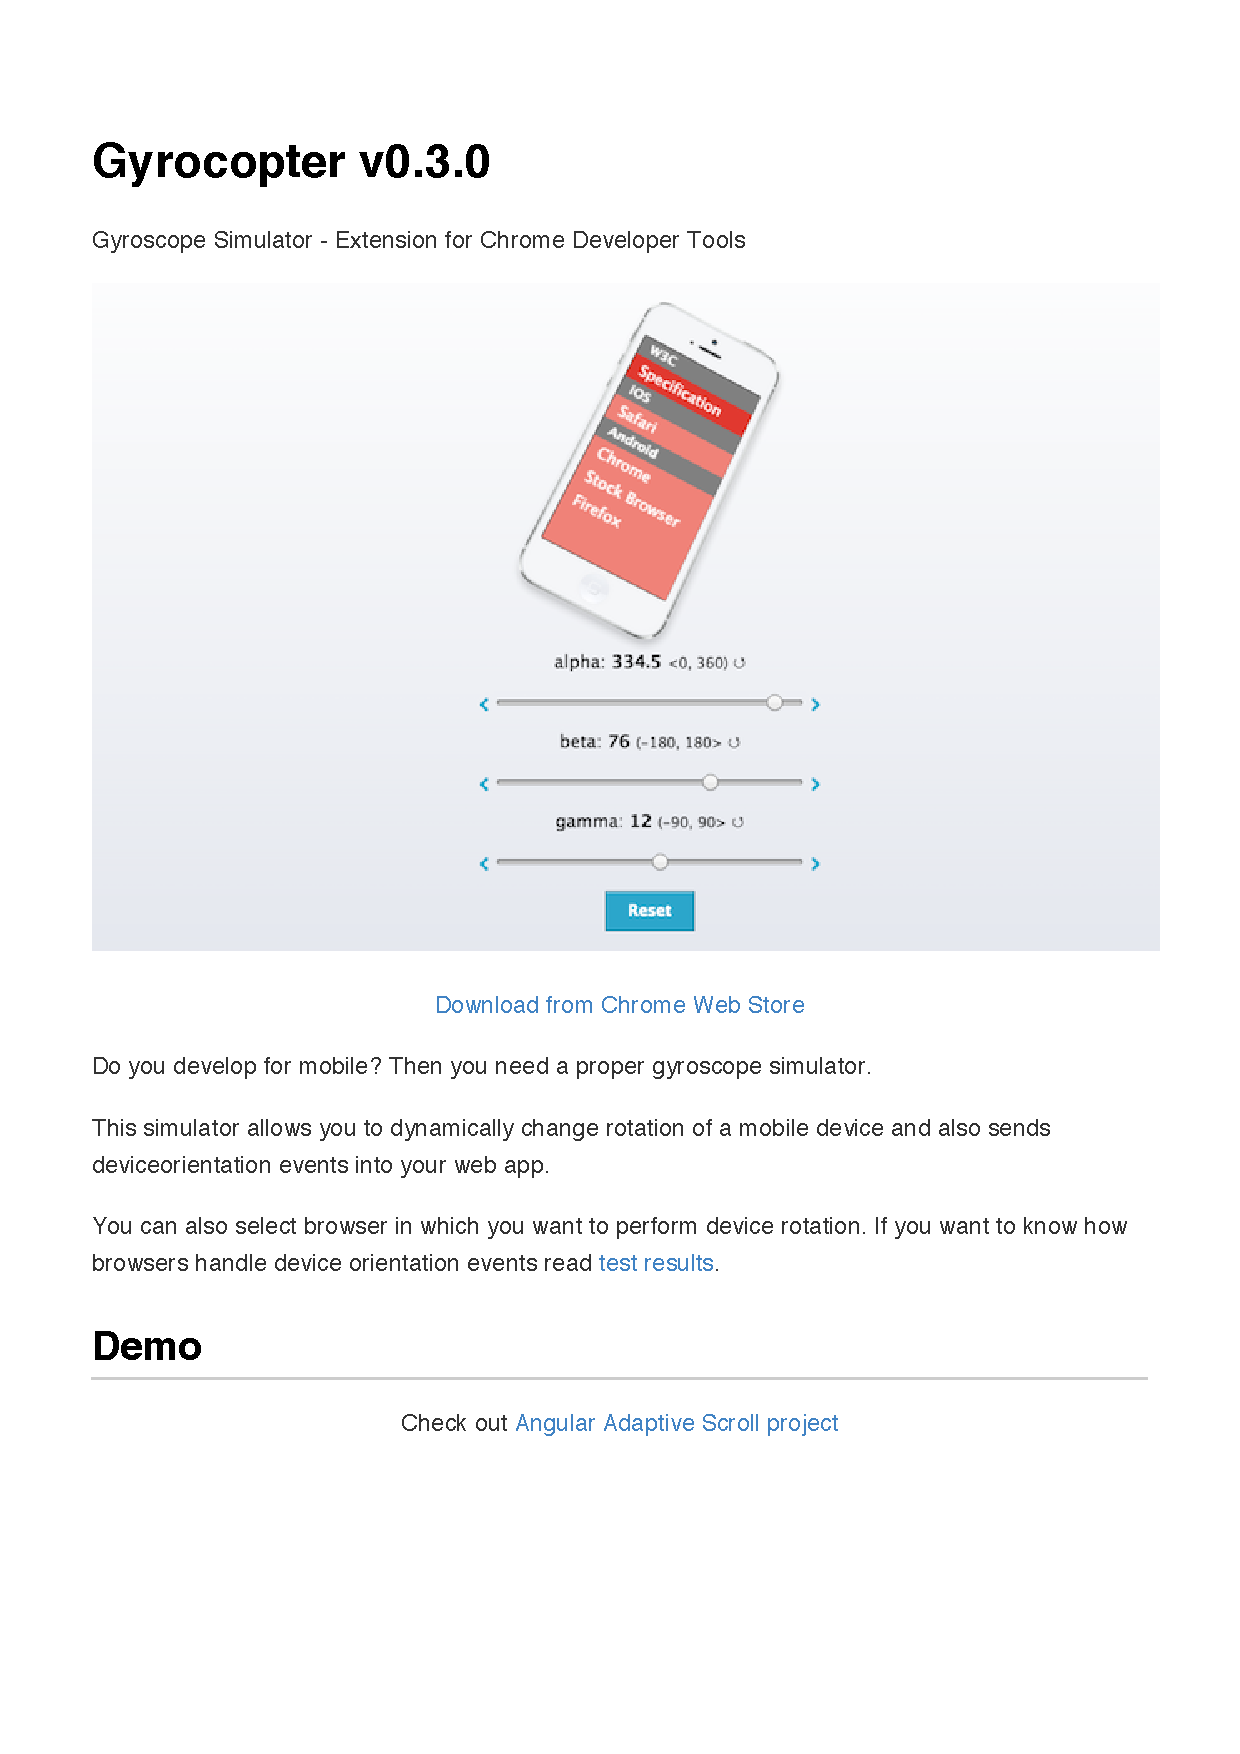
\includepdf[pages={1,2},scale=.8]{appendices/07-gyrocopter.pdf}
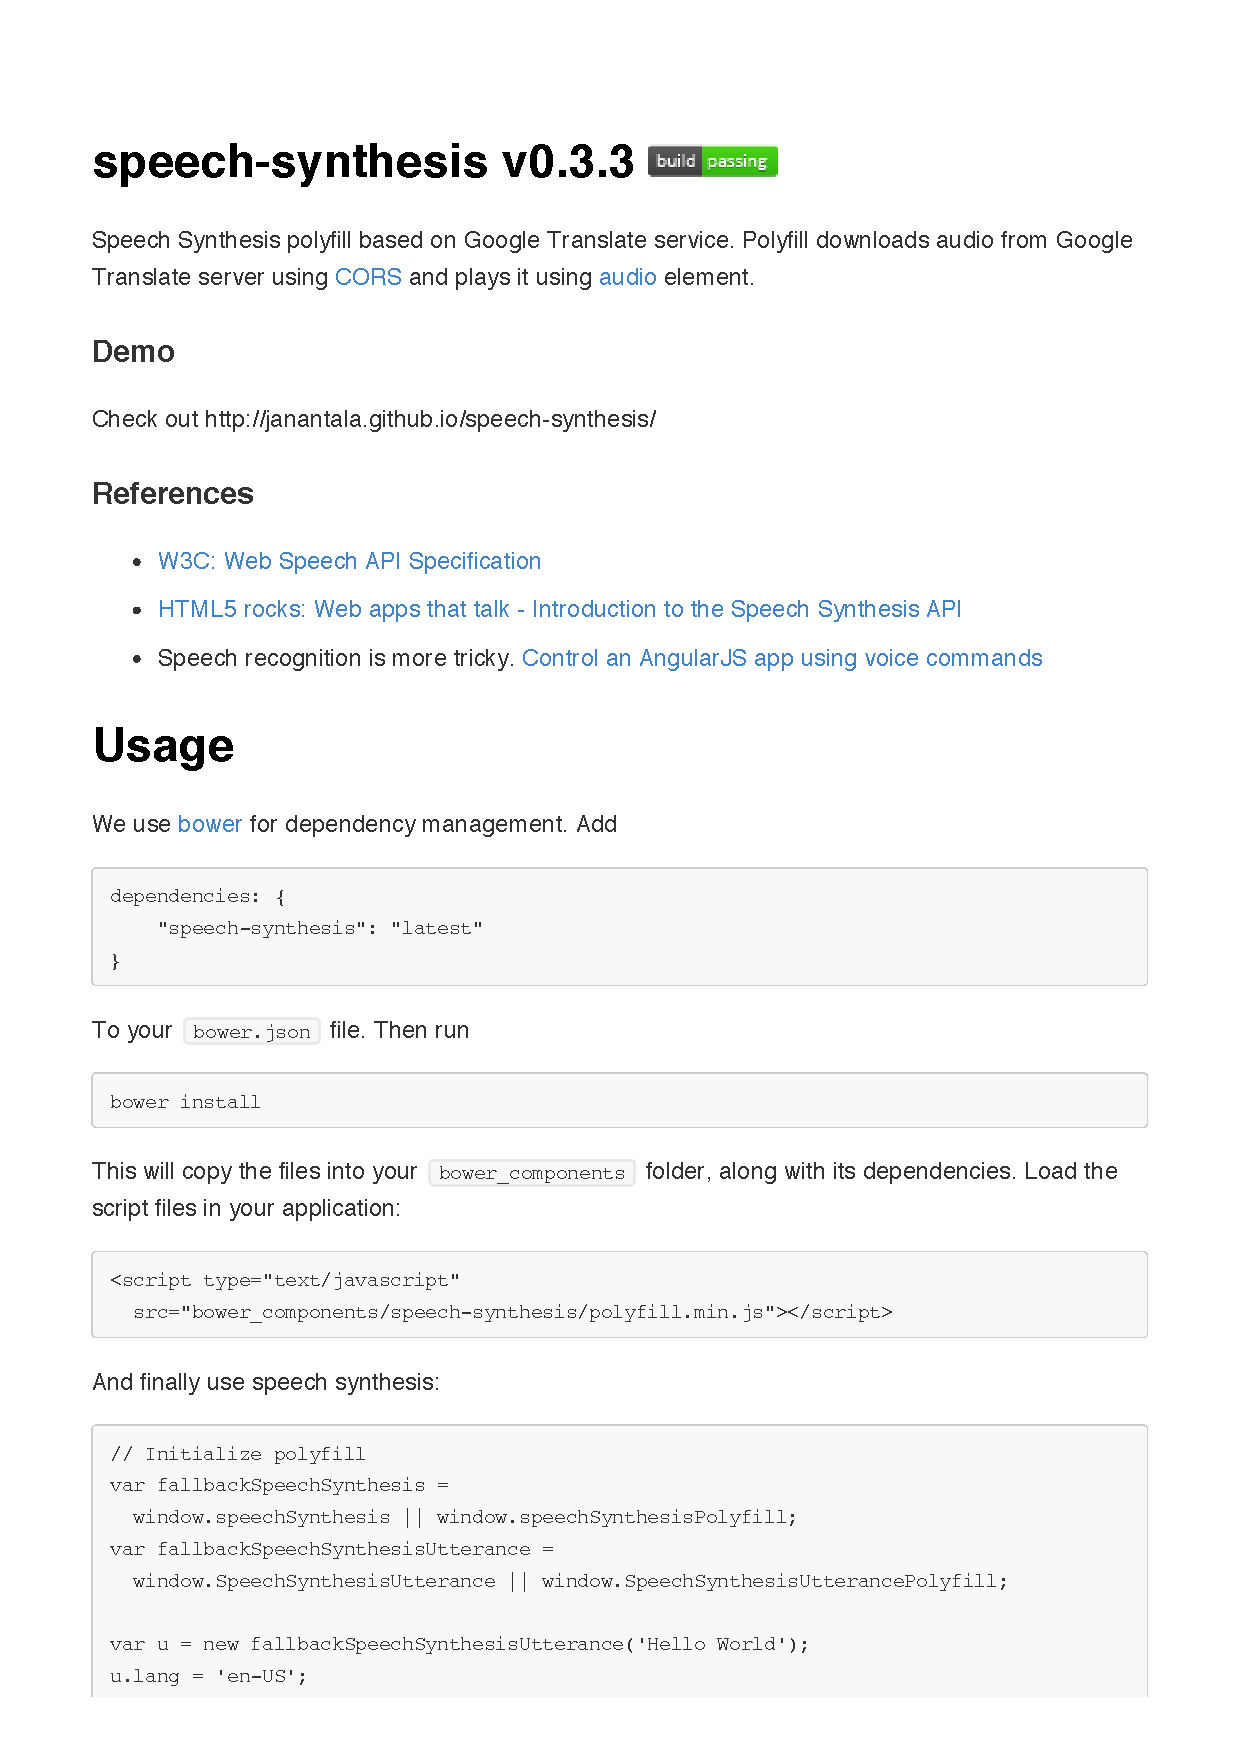
\includepdf[pages={1,2,3},scale=.8]{appendices/08-speechsynthesis.pdf}


% section technick_dokument_cia_a_in_tala_n_pr_ru_ka (end)

\newpage
\section{Článok prezentovaný na IIT.SRC2014} % (fold)
\label{sec:_l_nok_prezentovan_na_iit_src2014}

Na základe našej práce sme zároveň vytvorili odborný článok a prezentovali ho na konferencii IIT.SRC 2014 pod názvom ,,Beyond Adaptive Web Design''. V prílohe prinášame jeho plnú verziu.

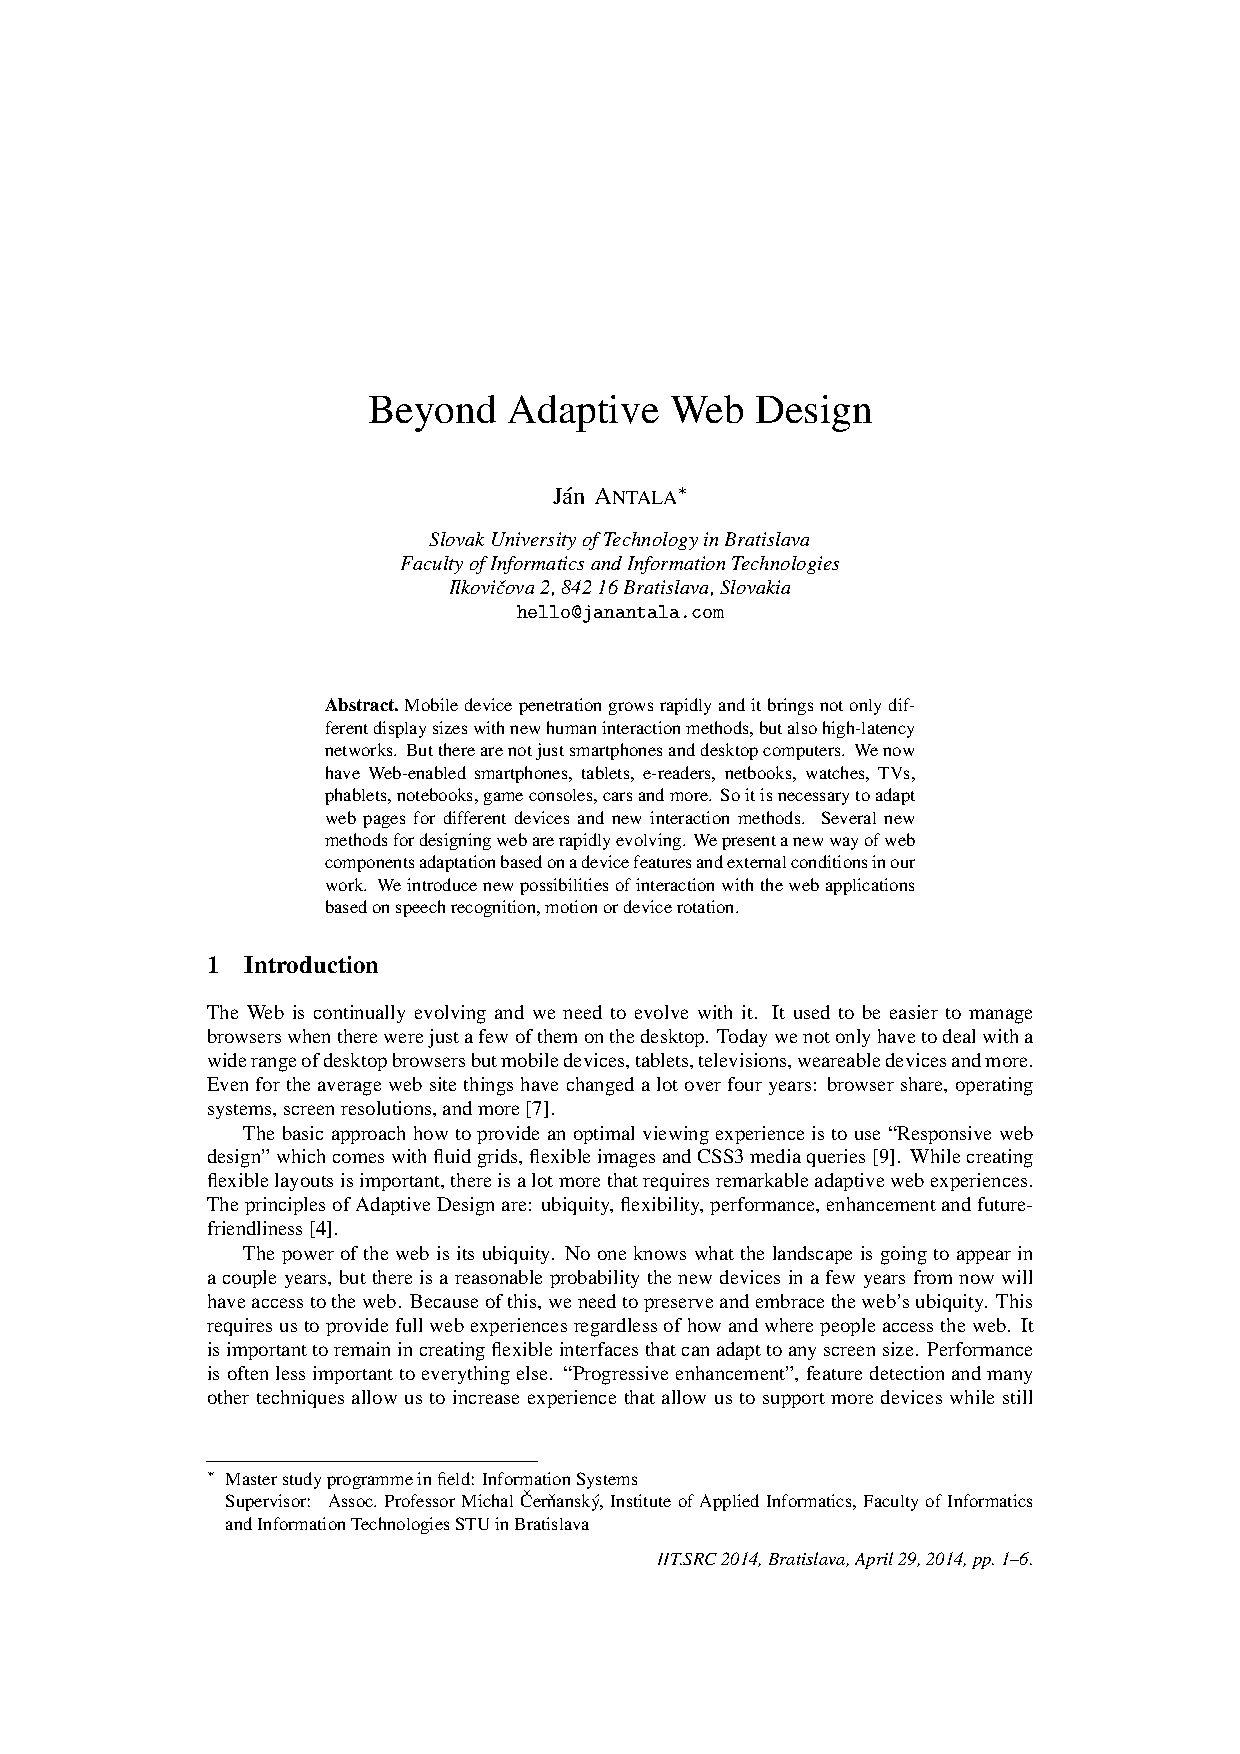
\includepdf[pages={1,2,3,4,5,6,7},scale=1.0]{appendices/paper.pdf}

% section _l_nok_prezentovan_na_iit_src2014 (end)
